\section{Recovering the multimodality}

In Section \ref{sec:action_multimodality}, we highlighted the difficulty of DP in modeling
the multimodal distribution of actions.
More specifically, we concluded that the method's suboptimality was due to non-expert and potentially
biased human demonstrations.
To address this, as we do not have access to expert demonstrations,
we decided to generate new trajectories to create a larger and more diverse dataset.
We first practiced on the PushT task before creating 50 new demonstrations each to reduce biases.
Once the new dataset was complete, we trained the model on these over 300 trajectories for 20k steps.

The effect of these new trajectories was immediate.
In Figure \ref{fig:multimodality_new}, we reproduced the previous singular case and generated 16
different trajectories from different noise vectors.
This time, we clearly see both trajectories emerging on either side of the T.
\begin{figure}[!htb]
    \centering
    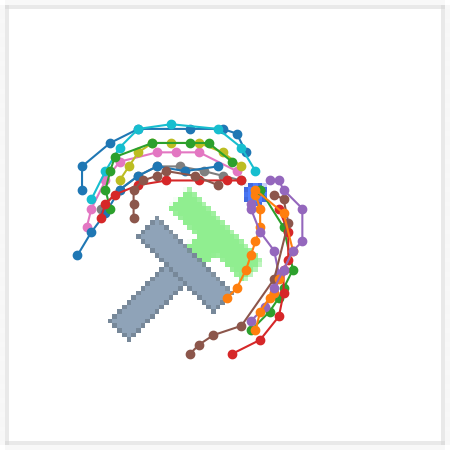
\includegraphics[width=0.6\linewidth]{figures/trajectories_multimodality.png}
    \caption{Illustration of the multimodal distribution of actions.}
    \label{fig:multimodality_new}
\end{figure}
To conclude on multimodality, DP is indeed capable of handling situations where multiple actions are possible,
unlike methods that rely on an L2 loss. However, the key to effectively modeling a multimodal distribution
lies in the training data. When a simulator is available, one option could be to generate new data
from existing data by applying geometric transformations or leveraging an expert policy trained through RL.